%%% causal_dag_tikz.tex — SCB Causal DAG (Direction D)
%%%
%%% PAPER PREAMBLE:
%%%   \usepackage{tikz}
%%%   \usetikzlibrary{arrows.meta, positioning, calc}
%%%
%%% STANDALONE PREVIEW:
%%%   pdflatex causal_dag_tikz.tex

\documentclass[tikz, border=4mm]{standalone}
\usetikzlibrary{arrows.meta, positioning, calc}

\begin{document}
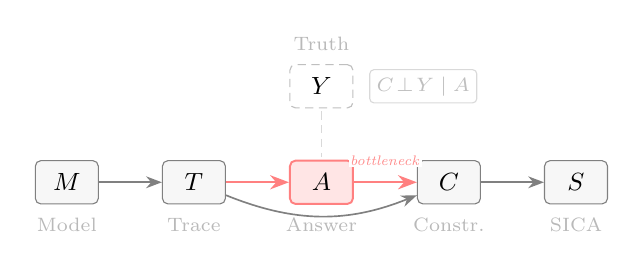
\begin{tikzpicture}[
  node distance=0.8cm,
  nd/.style={rectangle, rounded corners=2pt, draw=black!50,
             fill=gray!6, minimum height=5.5mm, minimum width=8mm,
             font=\small},
  bn/.style={nd, fill=red!10, draw=red!50, line width=0.7pt},
  ex/.style={nd, draw=gray!50, densely dashed, fill=white},
  >=Stealth,
  base/.style={->, semithick, black!50},
  leak/.style={->, line width=0.85pt, red!50},
  sub/.style={font=\scriptsize, text=gray!55},
]

% --- Nodes ---
\node[nd]             (M) {$M$};
\node[nd, right=of M] (T) {$T$};
\node[bn, right=of T] (A) {$A$};
\node[nd, right=of A] (C) {$C$};
\node[nd, right=of C] (S) {$S$};
\node[ex, above=0.65cm of A] (Y) {$Y$};

% --- Sub-labels ---
\node[sub, below=0.5mm of M] {Model};
\node[sub, below=0.5mm of T] {Trace};
\node[sub, below=0.5mm of A] {Answer};
\node[sub, below=0.5mm of C] {Constr.};
\node[sub, below=0.5mm of S] {SICA};
\node[sub, above=0.5mm of Y] {Truth};

% --- Causal edges ---
\draw[base] (M) -- (T);
\draw[leak] (T) -- (A);
\draw[leak] (A) -- (C);
\draw[base] (C) -- (S);
\draw[base, bend right=22] (T) to (C);

% --- Y ··· A (implicit: answer targets truth) ---
\draw[densely dashed, gray!30, shorten >=1pt, shorten <=1pt] (Y) -- (A);

% --- Bottleneck label on A->C ---
\node[font=\tiny, text=red!45, fill=white, inner sep=0.5pt]
  at ($(A)!0.5!(C) + (0, 0.27)$) {\textit{bottleneck}};

% --- d-separation annotation ---
\node[draw=gray!30, rounded corners=1.5pt, fill=white,
      inner sep=2.5pt, font=\scriptsize, text=gray!50,
      right=0.2cm of Y]
  {$C \!\perp\! Y \mid A$};

\end{tikzpicture}
\end{document}

%%% ==================== Figure for paper ====================
%%% Copy below into your .tex file.
%%%
%%% \begin{figure}[t]
%%% \centering
%%% \begin{tikzpicture}[
%%%   node distance=0.8cm,
%%%   nd/.style={rectangle, rounded corners=2pt, draw=black!50,
%%%              fill=gray!6, minimum height=5.5mm, minimum width=8mm,
%%%              font=\small},
%%%   bn/.style={nd, fill=red!10, draw=red!50, line width=0.7pt},
%%%   ex/.style={nd, draw=gray!50, densely dashed, fill=white},
%%%   >=Stealth,
%%%   base/.style={->, semithick, black!50},
%%%   leak/.style={->, line width=0.85pt, red!50},
%%%   sub/.style={font=\scriptsize, text=gray!55},
%%% ]
%%% \node[nd]             (M) {$M$};
%%% \node[nd, right=of M] (T) {$T$};
%%% \node[bn, right=of T] (A) {$A$};
%%% \node[nd, right=of A] (C) {$C$};
%%% \node[nd, right=of C] (S) {$S$};
%%% \node[ex, above=0.65cm of A] (Y) {$Y$};
%%%
%%% \node[sub, below=0.5mm of M] {Model};
%%% \node[sub, below=0.5mm of T] {Trace};
%%% \node[sub, below=0.5mm of A] {Answer};
%%% \node[sub, below=0.5mm of C] {Constr.};
%%% \node[sub, below=0.5mm of S] {SICA};
%%% \node[sub, above=0.5mm of Y] {Truth};
%%%
%%% \draw[base] (M) -- (T);
%%% \draw[leak] (T) -- (A);
%%% \draw[leak] (A) -- (C);
%%% \draw[base] (C) -- (S);
%%% \draw[base, bend right=22] (T) to (C);
%%%
%%% \draw[densely dashed, gray!30, shorten >=1pt, shorten <=1pt] (Y) -- (A);
%%%
%%% \node[font=\tiny, text=red!45, fill=white, inner sep=0.5pt]
%%%   at ($(A)!0.5!(C) + (0, 0.27)$) {\textit{bottleneck}};
%%%
%%% \node[draw=gray!30, rounded corners=1.5pt, fill=white,
%%%       inner sep=2.5pt, font=\scriptsize, text=gray!50,
%%%       right=0.2cm of Y]
%%%   {$C \!\perp\! Y \mid A$};
%%% \end{tikzpicture}
%%% \caption{Causal DAG of the SCB pipeline. The dashed link indicates
%%%   that answer~$A$ implicitly targets ground truth~$Y$; all
%%%   information about~$Y$ reaching constraints~$C$ is mediated
%%%   by~$A$ ($C \perp Y \mid A$), making self-verification
%%%   inherently answer-biased.}
%%% \label{fig:causal-dag}
%%% \end{figure}
